\chapter{Logistic Regression}

\section{Classification}

The classification problem is just like the regression problem, except that the values we now want to predict take on only a small number of discrete values. For now, we will focus on the binary classification problem in which \textbf{y} can take on only two values, 0 and 1. (Most of what we say here will also generalize to the multiple-class case.) For instance, if we are trying to build a spam classifier for email, then $ x^{(i)} $ may be some features of a piece of email, and y may be 1 if it is a piece of spam mail, and 0 otherwise. Hence, y $\in$ {0,1}. 0 is also called the negative class, and 1 the positive class, and they are sometimes also denoted by the symbols “-” and “+.” Given $ x^{(i)} $, the corresponding $ y^{(i)} $ is also called the label for the training example.

\subsection{Hypothesis Representation}

We could approach the classification problem ignoring the fact that y is discrete-valued, and use our old linear regression algorithm to try to predict y given x. However, it is easy to construct examples where this method performs very poorly. Intuitively, it also doesn’t make sense for $ h_\theta (x) $ to take values larger than 1 or smaller than 0 when we know that y $\in$ {0, 1}. To fix this, let’s change the form for our hypotheses $ h_\theta (x) $ to satisfy $ 0 \leq h_\theta (x) \leq 1 $. This is accomplished by plugging $ \theta^Tx $ into the Logistic Function (also called Sigmoid Function).\\


\begin{tcolorbox}[width=\textwidth,colback={white},colbacktitle=white]
\begin{align*}
h_\theta(x) &=g(\theta^Tx)\\
z &=\theta^Tx\\
g(z) &=\frac{1}{1+e^{-z}}
\end{align*}
\end{tcolorbox} 

\pagebreak

The following image shows us what the sigmoid function looks like:

\begin{figure}[h!]
	\centering
	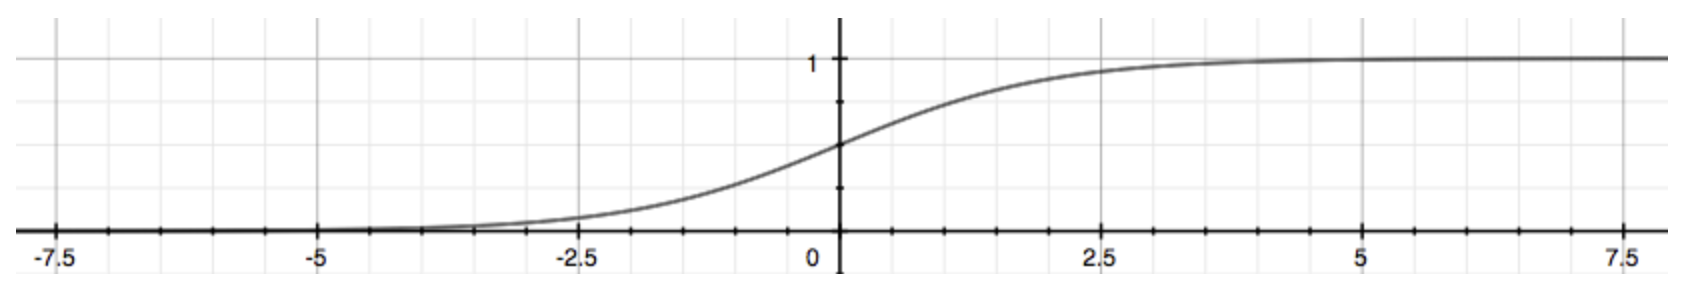
\includegraphics[width=1\textwidth]{fig/sigmoide}
	\caption{Sigmoid function}
\end{figure}

The function $ g(z) $, shown here, maps any real number to the (0, 1) interval, making it useful for transforming an arbitrary-valued function into a function better suited for classification.\\

$\mathbf{ h_\theta(x)  }$ \textbf{will give us the probability that our output is 1.} For example, $ h_\theta(x)=0.7 $ gives us a probability of 70\% that our output is 1. Our probability that our prediction is 0 is just the complement of our probability that it is 1 (e.g. if probability that it is 1 is 70\%, then the probability that it is 0 is 30\%).

\subsection{Decision Boundary}

In order to get our discrete 0 or 1 classification, we can translate the output of the hypothesis function as follows:

\begin{tcolorbox}[width=\textwidth,colback={white},colbacktitle=white]
	\begin{align*}
	When \hspace{0.2cm} z \geq 0  \hspace{0.2cm} \Rightarrow \hspace{0.2cm} h_\theta(x) & \geq 0.5 \rightarrow y=1\\
	When \hspace{0.2cm} z \leq 0  \hspace{0.2cm} \Rightarrow \hspace{0.2cm} h_\theta(x) & \leq 0.5 \rightarrow y=0
	\end{align*}
\end{tcolorbox} 

So if our input to g is $ \theta^T X $, then that means:

\begin{align*}
&h_\theta(x)=g(\theta^Tx) \geq 0.5 \\
&When \hspace{0.2cm} \theta^Tx \geq 0
\end{align*}

From these statements we can now say:

\begin{align*}
\theta^Tx \geq 0 &\Rightarrow y=1\\
\theta^Tx < 0 &\Rightarrow y=0
\end{align*}

The decision boundary is the line that separates the area where \textbf{y = 0 }and where \textbf{y = 1}. It is created by our hypothesis function.

\subsection{Cost Function}

We cannot use the same cost function that we use for linear regression because the Logistic Function will cause the output to be \textbf{wavy}, causing many local optima. In other words, \textit{it will not be a convex function}.

Instead, our cost function for logistic regression looks like:

\begin{equation}
J(\theta)=\frac{1}{m}\sum_{i=1}^{m}Cost\left(h_\theta(x^{(i)}),  y^{(i)}\right)
\end{equation}

Where:

\begin{align}
Cost\left(h_\theta(x^{(i)}),  y^{(i)}\right) &= -log(h_\theta(x)) &if \hspace{0.35cm} y = 1\\
Cost\left(h_\theta(x^{(i)}),  y^{(i)}\right)& = -log(1-h_\theta(x)) & if \hspace{0.35cm} y = 0
\end{align}

\begin{figure}[h!]
	\centering
	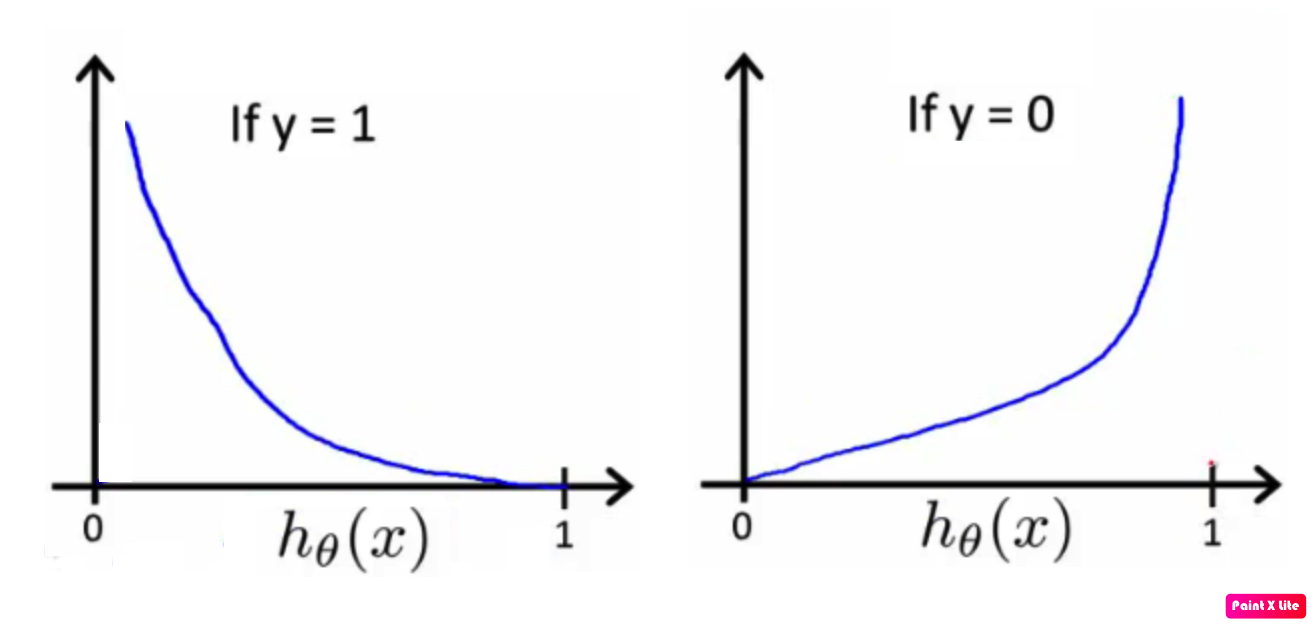
\includegraphics[width=1\textwidth]{fig/cost_logistic}
	\caption{When \textbf{y = 1 (left)}, \textbf{y = 0 (right)} we get the following plot for J($ \theta $) vs $ h_\theta (x) $}
	\label{fig:logistic}
\end{figure}

If our correct answer 'y' is 0, then the cost function will be 0 if our hypothesis function also outputs 0. If our hypothesis approaches 1, then the cost function will approach infinity.\\

If our correct answer 'y' is 1, then the cost function will be 0 if our hypothesis function outputs 1. If our hypothesis approaches 0, then the cost function will approach infinity.\\

We can compress our cost function's two conditional cases into one case:

\begin{equation}
Cost(h_\theta(x^{(i)}),  y^{(i)}) = -y\cdot log(h_\theta(x)) -(1-y)\cdot log(1-h_\theta(x)) 
\end{equation}

We can fully write out our entire cost function as follows:

\begin{center}
$$J(\theta) = -\frac{1}{m}\sum_{i=1}^{m}\left[y^{(i)}\cdot log(h_\theta(x^{(i)})) +(1-y^{(i)})\cdot log(1-h_\theta(x^{(i)}))\right] $$
\end{center}

A vectorized implementation is:

\begin{align*}
h&=g(X\theta) \\
J(\theta)&=\frac{1}{m}\cdot(-y^T\cdot log(h)-(1-y)^T\cdot log(1-h))
\end{align*}

\subsection{Gradient Descent}

The general form of gradient descent is:

\begin{align*}
Repeat &: \{\\
\theta_j &:= \theta_j - \alpha \frac{\partial}{\partial \theta_j} J(\theta_0, \theta_1) \\
 &   \}
\end{align*}

We can work out the derivative part using calculus to get:


\begin{align*}
Repeat &: \{\\
\theta_j &:= \theta_j-\alpha \frac{1}{m} \sum_{i=1}^{m}\left(h_\theta(x^{(i)})-y^{(i)}\right)\cdot x^{(i)}_j \\
&   \}
\end{align*}

\textbf{Notice that this algorithm is identical to the one we used in linear regression. We still have to simultaneously update all values in theta.}\\

A vectorized implementation is:\\

\begin{center}
$\theta:=\theta- \frac{\alpha}{m} X^T \left(g(X\theta)- \overrightarrow{y}\right)$
\end{center}

\section{Multiclass Classification: One-vs-all}

Now we will approach the classification of data when we have more than two categories. Instead of y = {0,1} we will expand our definition so that y = {0,1...n}.\\

Since y = {0,1...n}, we divide our problem into n+1 (+1 because the index starts at 0) binary classification problems; in each one, we predict the probability that 'y' is a member of one of our classes.\\

\begin{tcolorbox}[width=\textwidth,colback={white},colbacktitle=white]
	\begin{align*}
	&y \in \{0,1 \dots n\}\\
	&h^{(0)}_\theta(x)=P(y=0|x;\theta)\\
	&h^{(1)}_\theta(x)=P(y=1|x;\theta)\\
	&\dots\\
	&h^{(n)}_\theta(x)=P(y=n|x;\theta)\\
	&prediction = \underset{i}max(h^{(i)}_\theta(x))
	\end{align*}
\end{tcolorbox} 

We are basically choosing one class and then lumping all the others into a single second class. We do this repeatedly, applying binary logistic regression to each case, and then use the hypothesis that returned the highest value as our prediction.\\

The following image shows how one could classify 3 classes:\\

\begin{figure}[h!]
	\centering
	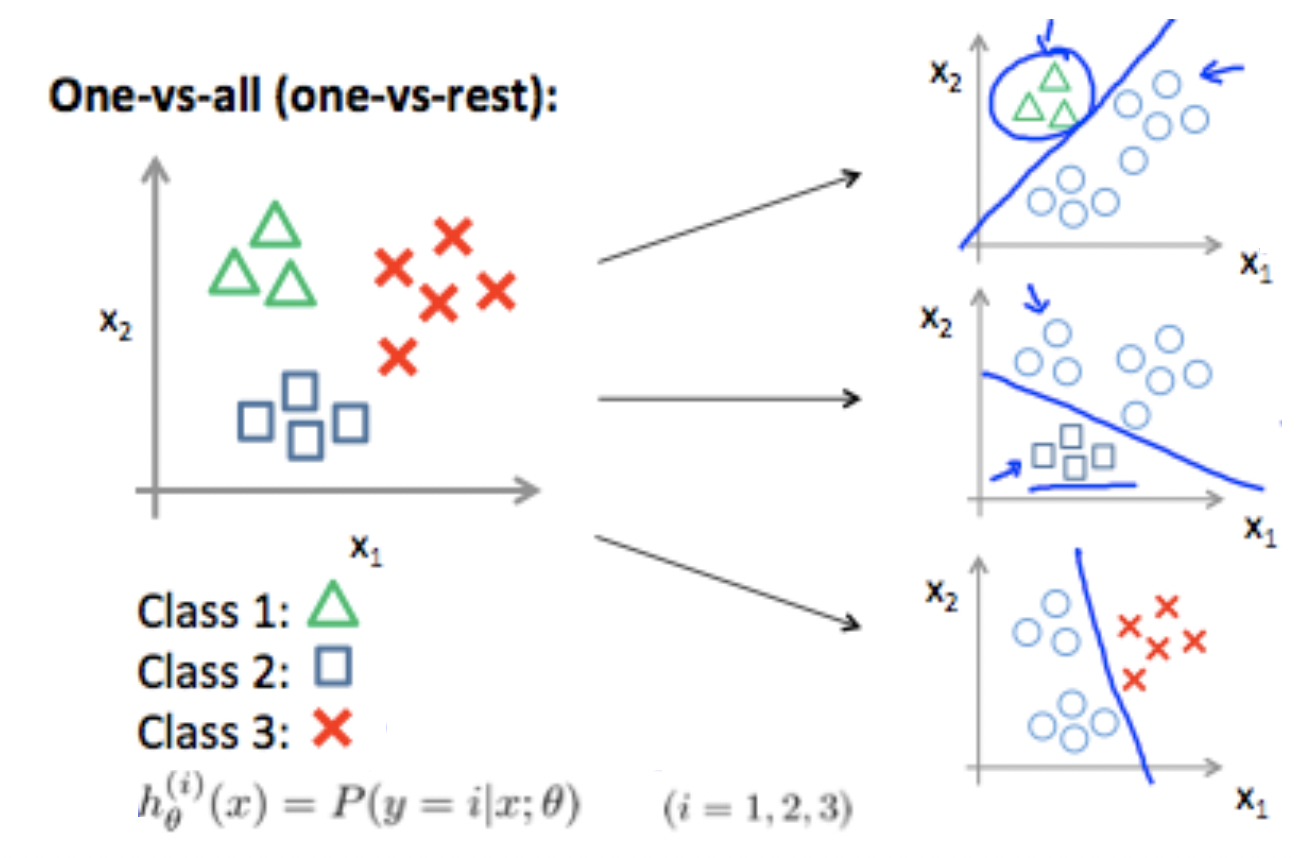
\includegraphics[width=0.65\textwidth]{fig/onvsall}
	\caption{One-vs-all or One-vs-Rest}
\end{figure}